\section{Softwaretests in Verbindung mit Unity}
\label{sec:testing}

In den vorhergehenden Kapiteln wurden die verschiedenen Funktionalitäten des Spiels ausführ\-lich beschrieben. Um das Vertrauen in die eigene Arbeit zu erhöhen und Fehler im Zuge des Entwicklungsprozesses frühzeitig identifizieren zu können, ist die Erstellung und Durchführung von Softwaretests ein weiterer wichtiger Bestandteil des Projekts. 

%Bei der Entwicklung von Software ist Testen aus vielerlei Gründen eine wichtige Aufgabe. Unter anderem wird hierdurch das Vertrauen in die eigene Arbeit erhöht, da fehleranfällige Stellen zu einem frühen Zeitpunkt im Entwicklungsprozess identifiziert werden. Des Weiteren wird in vielen Projekten ein gewisser Erfüllungsgrad verschiedenster Testmetriken vonseiten der Auftraggeber gefordert, um das Vertrauen in das entwickelte Produkt auch auf Gegenseite herzustellen. 

Im Folgenden wird die Durchführung von zweierlei Arten von Tests beschrieben, die bei der Entwicklung des Projekts zum Einsatz kommen. Zunächst wird hierbei auf automatisierte Modultests inklusive deren Besonderheiten in Verbindung mit dem Unity Framework eingegangen. Anschließend werden verschiedene manuelle Tests vorgestellt, die im Zuge des Projekts durchgeführt werden.  

\subsection{Modultests}

Um die einwandfreie Funktionalität des implementierten Quellcodes bereits zur Entwicklungszeit
sicherstellen zu können, wurden automatisierte Modultests parallel zum eigentlichen
Programmcode entwickelt. Die Verwendung des Unity Frameworks erforderte hierbei ein vom Standard abweichendes Vorgehen, welches im Nachfolgenden näher erläutert wird. Hierbei wird zunächst auf die allgemeine Vorgehensweise zur Erstellung von Modultests unter Unity eingegangen. Anschließend werden Problemstellungen erläutert, die sich daraus ergeben, und zwei Lösungsansätze dafür aufgezeigt. Abschließend wird eine Übersicht bezüglich der Testabdeckung innerhalb des Projekts gegeben. 

\subsubsection{Allgemeines zu Modultests in Unity}

%https://de.slideshare.net/MikkoMcMenamin/unit-testing-in-unity-128173223


Das Unity Framework unterstützt Entwickler bei der Erstellung von Modultests durch die Bereitstellung einer Test Applikation, dem \textit{Unity Test Runner} (siehe Abb. \ref{fig:unity_test_runner}). Dieser ist ein grafisches Werkzeug, das die Ausführung von Testfällen per Knopfdruck ermöglicht und eine visuelle Rückmeldung bezüglich der einzelnen Ergebnisse liefert. 

%\vspace{1em}
%\begin{minipage}{\linewidth}
%	\begin{center}
      \begin{figure}[!t]
      \begin{center}
		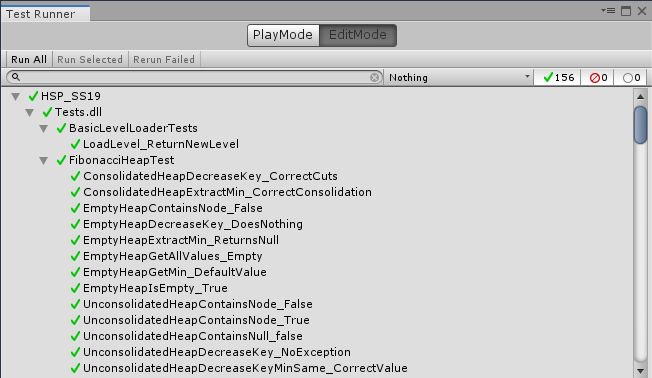
\includegraphics[width=1.00\linewidth]{pics/unity_test_runner.png}
		\captionof{figure}[Grafische Oberfläche des Unity Test Runners]{Grafische Oberfläche des Unity Test Runners}
		\label{fig:unity_test_runner}
		  \end{center}
		\end{figure}
%	\end{center}
%\end{minipage}

Wie in Abbildung \ref{fig:unity_test_runner} zu erkennen ist, können Testfälle in die beiden Kategorien \textit{PlayMode} und \textit{EditMode} unterteilt werden. Die Zuordnung erfolgt durch eine entsprechende Annotation über der Signatur einer Testmethode. Modultests, die als \textit{EditMode} deklariert sind, stellen die leichtgewichtigere Variante dar. Diese Testmethoden entsprechen dem auch außerhalb von Unity üblichen Verständnis von Modultests. Bei der Ausführung der Tests werden diese direkt im Editor-Modus von Unity durchgeführt. Spezielle Methoden von Spielobjekten, wie beispielsweise \texttt{Update()}, \texttt{Awake()} und \texttt{Start()} werden hierbei nicht aufgerufen. Tests, die im \textit{EditMode} ausgeführt werden, benötigen daher wenig Zeit zur Durchführung und sind äußerst performant. Ihr Einsatz zielt in erster Linie auf die Überprüfung einzelner isolierter Methoden ab, die ein gleichbleibendes Verhalten aufweisen und nicht von mehreren aufeinanderfolgenden Einzelbildern oder der Unity Spieleengine abhängen. Ein Beispiel hierfür ist die Funktionalität einer Datenstruktur. Im Gegensatz hierzu wird bei jeder als \textit{PlayMode} Test deklarierten Methode eine komplette Spielszene innerhalb der Unity-Engine geladen und alle oben genannten Methoden werden für jedes Spielobjekt ausgeführt. Das System verhält sich bei der Ausführung eines \textit{PlayMode} Tests exakt so, als würde ein Benutzer die Unity Applikation starten und die jeweilige Methode ausführen. Dies resultiert in lang andauernden Prozessen, die eher zur Überprüfung dynamischer Spielinhalte über mehrere Einzelbilder hinweg oder auch zur Überprüfung bestimmter Eigenschaften erzeugter Spielobjekte geeignet sind. Durch \textit{PlayMode} Tests lassen sich beispielsweise Testfälle konstruieren, die die Bewegung eines Spielobjekts über den Bildschirm verfolgen und innerhalb eines jeden Einzelbilds die tatsächliche Position des Objekts mit der kalkulierten, erwarteten Position vergleichen. Die Einsatzbereiche der beiden Varianten von Modultests sind nicht klar abgegrenzt. Die Vor- und Nachteile müssen für jede Funktionalität gegenübergestellt und auf ihre Verwendbarkeit hin untersucht werden.  

%- Play Mode: Unity Engine wird gesteartet
%- Play Mode: Auch hier können keine MonoBehaviours instanziiert werden. Entweder leeres Spielobjekt usw. , oder ganze Szene laden!
%- Play Mode: Möglichkeit 2: Ganze Szene wird geladen! Mit allen !!!Spielobjekten, etc. => Keine isolierten Tests von kleinen Komponenten! Modultests => kleinste Module => Methoden!
%
%- PlayMode Tests testen ganze Abläufe, sind sehr langsam. 




Zur Implementierung der Modultests wird die Open-Source Bibliothek NUnit\footnote{https://nunit.org/} verwendet. Durch Annotation der Methoden innerhalb einer Testklasse lassen sich diese Methoden in unterschiedliche Kategorien mit verschiedenen Verwendungszwecken einteilen. In Tabelle \ref{tab:nunit_annotations} sind die wichtigsten Annotationen der NUnit Bibliothek mit ihren zugehörigen Bedeutungen beschrieben. Des Weiteren bietet NUnit vielfältige Möglichkeiten in Form von statischen Methoden, um erwartete mit tatsächlichen Ergebnissen zu vergleichen oder auch bestimmte Eigenschaften von Resultaten zu überprüfen. 

%- Wichtige Annotationen


\begin{table}[t!]
\caption[Häufig genutzte Annotationen der NUnit Bibliothek mit zugehöriger Bedeutung]{Häufig genutzte Annotationen der NUnit Bibliothek mit zugehöriger Bedeutung}
\begin{center}
\begin{tabular}{|l|l|}
\hline
  Annotation & Beschreibung \\
  \hline
  \texttt{$[$Test$]$} & Kennzeichnet eine Methode innerhalb einer Testklasse als Test. \\
  \texttt{$[$TestCase$]$} & Ermöglicht die mehrmalige Ausführung einer Testmethode mit \\ 
  &	verschiedenen Argumenten. \\
  \texttt{$[$SetUp$]$} & Kennzeichnet eine Methode, die \textbf{vor jedem} Test einer Testklasse \\
  & aufgerufen wird. \\
  \texttt{$[$TearDown$]$} & Kennzeichnet eine Methode, die \textbf{nach jedem} Test einer Testklasse \\
  & aufgerufen wird.  \\
  \texttt{$[$OneTimeSetUp$]$} & Kennzeichnet eine Methode, die \textbf{einmalig vor allen} Tests einer \\
  & Testklasse ausgeführt wird. \\ 
  \texttt{$[$OneTimeTearDown$]$} & Kennzeichnet eine Methode, die \textbf{einmalig nach allen} Tests einer \\
  & Testklasse ausgeführt wird.  \\
  \hline
\end{tabular}
\label{tab:nunit_annotations}
\end{center}
\end{table}

%=>> Wichtige Methoden (Assert, etc.) ???

Bei der Erstellung von Modultests muss berücksichtigt werden, dass viele zu testende Module aufgrund von äußeren Abhängigkeiten nicht beziehungsweise nur schwer isoliert getestet werden können. Diese Abhängigkeiten können beispielsweise Eingabeparameter sein, die über spezielle Eigenschaften verfügen, welche dann in einer konkreten Testmethode zur Steuerung des Kontrollflusses verwendet werden. Um eine funktionale Komponente so isoliert wie nur möglich testen zu können, muss daher in vielen Fällen die Umgebung der zu testenden Funktionalität künstlich nachgebildet werden. Dies geschieht durch die Verwendung von Platzhalter-Objekten, auch \textit{Mocks} genannt, die anstelle von realen Instanzen der notwendigen Klassen verwendet werden. In diesem Projekt wird hierfür die Bibliothek NSubsitute\footnote{https://nsubstitute.github.io/} verwendet. 

Ein weitverbreitetes Vorgehen bei der Erstellung von Modultests ist die Strukturierung der inneren Funktionalität einer Testmethode in drei klar voneinander abgegrenzte Bereiche. Diese Bereiche werden als \textit{Vorbereitung}, \textit{Aktion} und \textit{Bestätigung} bezeichnet. Im ersten Abschnitt werden alle Objekte, die für den Aufruf der zu testenden Methode notwendig sind, initialisiert und die Werte der Daten festgelegt, die an die zu testende Methode übergeben werden. Anschließend wird die zu testende Methode mit den vorbereiteten Daten aufgerufen. Im dritten Bereich wird überprüft, ob das Ergebnis der zu testenden Methode mit dem erwarteten Ergebnis übereinstimmt. Dieses Vorgehen wird, in Anlehnung an die Anfangsbuchstaben der englischen Bezeichnungen der einzelnen Bereiche \textit{Arrange}, \textit{Act} und \textit{Assert}, auch als \textit{AAA}-Muster bezeichnet. Auch in diesem Projekt werden die Testmethoden nach dieser Struktur entwickelt. 

%\begin{tabular}[t]{ll}
%%\tabitem 
%\textbf{Wand:} & Position\\
%\textbf{Tür:} & Position, Rotation\\
%\textbf{Waffe:} & Position, Rotation, Typ, Munitionsmenge\\
%\textbf{Gegner:} & Position, Typ, Patrouillenpunkte, Waffentyp, Munitionsmenge\\
%\textbf{Ziel:} & Position\\
%\textbf{Level:} & Größe, Startposition, Aktuelle Position
%\end{tabular}


\subsubsection{Schwierigkeiten bei der Erstellung der Modultests}

Die Entwicklung von Modultests in Unity Projekten ist mit verschiedenen Herausforderungen verbunden, die in Projekten außerhalb der Unity-Engine nicht existieren. Diese resultieren aus dem von Unity festgelegten Zusammenspiel zwischen Spielobjekten, Verhaltensklassen, die diesen Spielobjekten als Komponenten hinzugefügt werden können, und den logischen Abhängigkeiten innerhalb dieser Klassen.

Die größte Herausforderung stellt hierbei das Testen von Klassen dar, die von der Unity eigenen Basisklasse \textit{MonoBehaviour} erben. Da jede Klasse, die einem Spielobjekt als Komponente hinzugefügt werden soll, von \textit{MonoBehaviour} erben muss, ist die Zahl dieser abgeleiteten Klassen innerhalb eines Unity Projekts sehr groß. 

Dies bringt verschiedene Probleme mit sich. Zum einen lassen sich von \textit{MonoBehaviour} abgeleitete Klassen nicht auf Ebene des Quellcodes instanziieren. Dies ist allerdings eine Grundvoraussetzung, um im Aktionsbereich eines Modultests eine zu testende Methode dieser Klasse aufrufen zu können. Zum anderen können Klassen dieses Typs auch nicht durch Platzhalter Objekte nachgebildet werden. Dies hat zur Konsequenz, dass die Umgebungen von Klassen, die selbst zwar nicht von \textit{MonoBehaviour} erben, aber Abhängigkeiten zu solchen abgeleiteten Klassen besitzen, nur sehr schwer und stellenweise unmöglich nachzustellen sind.

Die Tatsache, dass von \textit{MonoBehaviour} abgeleitete Klassen nicht instanziiert werden können, bringt auch weiterführende Probleme in Hinblick auf statistische Aspekte im Zuge der Qualitätssicherung mit sich. Herkömmliche Werkzeuge zur Überprüfung der Testabdeckung und Ermittlung verschiedener Testmaße lassen sich nicht mehr ohne Weiteres benutzen, da die implementierten Testmethoden vom Standard abweichend entwickelt werden müssen, um ausgeführt werden zu können. 

Eine weitere Herausforderung im Zuge des Entwicklungsprozesses ist die Durchführung von \textit{PlayMode} Testfällen. Da zu Beginn eines jeden Testfalls eine komplette Spielszene innerhalb der Unity-Engine geladen wird, ist die Ausführung dieser Tests sehr rechen- und zeitintensiv. Bereits wenige Testfälle genügen, um eine länger andauernde Testphase zu verursachen. Mit steigender Anzahl an Testfällen nimmt die benötigte Zeit schnell zu, wodurch eine iterative Durchführung im laufenden Entwicklungsprozess erschwert wird. 

%- Klassen, die von MonoBehaviour erben -> Wieso sind die ein Problem? -> Begründung! (Kann man nicht instanziieren, ...) => WARNUNG, kein ERROR!
%
%- Kann man nicht mit NSubstitute mocken!
%
%- Warum nicht Play Mode Tests: jedes Mal wird die ganze Unity Engine gestartet! => Im laufenden Entwicklungsprozess zu aufwändig für jede kleine Komponente!
%
%- Testabdeckung mit herkömmlichen Tools nicht möglich

\subsubsection{Beschreibung verschiedener Lösungsansätze zum Testen von MonoBehaviours}
\label{chapter:mono_beh_testen_loesungen}

Es existieren zwei unterschiedliche Ansätze, um von \textit{MonoBehaviour} abgeleitete Klassen zu testen. Bei ersterer Möglichkeit werden einer Testklasse zwei private Attribute hinzugefügt, wobei ein Attribut vom Typ \texttt{GameObject} und das andere vom Typ der Klasse sein muss, deren Funktionalität überprüft werden soll. Anschließend wird ein neues \texttt{GameObject} instanziiert und die Referenz dem entsprechenden Attribut zugewiesen. Dem neu erstellten, leeren Spielobjekt wird nun die Klasse mit der zu testenden Funktionalität als Komponente hinzugefügt. Der Rückgabewert dieser Methode wird in dem dazugehörigen Attribut abgespeichert. Ab diesem Zeitpunkt ist es möglich, alle öffentlichen Methoden der Klasse aufzurufen, welche die zu testende Funktionalität enthält. Da das soeben beschriebene Vorgehen zu Beginn einer jeden Testmethode ausgeführt werden muss, bietet es sich an, den hierfür notwendigen Programmcode in eine eigene Methode auszulagern und diese mit der NUnit Annotation \texttt{OneTimeSetUp} zu kennzeichnen. Die Methode wird hierdurch einmalig zu Beginn der Testphase ausgeführt und die gesetzten, privaten Attribute können in allen folgenden Testmethoden verwendet werden. 

Eine weitere Möglichkeit zur Lösung des Problems ist die Anwendung des \textit{Humble Object Pattern} \cite{xUnit_Test_Patterns_Refactoring}. Gerard Meszaros beschreibt in seinem Lehrbuch sieben unterschiedliche Varianten dieses Entwurfsmusters, die sich je nach konkretem Anwendungsfall unterscheiden. Im Folgenden wird lediglich die für das Projekt relevante Variante näher beschrieben, für eine ausführliche Erläuterung der übrigen Optionen siehe \cite{xUnit_Test_Patterns_Refactoring}.

Die grundlegende Idee des Entwurfsmusters ist es, den Programmcode, der die eigentliche Logik ausführt, in eine neue Komponente auszulagern und diese isoliert zu testen. Eine Visualisierung dieser Vorgehensweise ist in Abbildung  \ref{fig:humble_object_pattern} dargestellt. Anstatt die zu testende Komponente mit ihren Abhängigkeiten direkt zu testen (Abb. \ref{fig:humble_01}) wird die relevante Logik in eine neue Komponente verlagert und dort getestet (Abb. \ref{fig:humble_02}). Das \textit{Humble Objekt} agiert dann nur noch als eine Art Vermittlerschicht, die die isolierte Funktionalität dieser Komponente aufruft und die Rückgabewerte weiterverarbeitet. Innerhalb des \textit{Humble Objekts} wird wenig eigener Quellcode benötigt. Es ist lediglich für die Bereitstellung der benötigten Informationen beim Aufruf der ausgelagerten Methoden verantwortlich. Da der übrige Quellcode innerhalb eines \textit{Humble Objekts} vor allem die Interaktion des Objekts mit seiner Umwelt zum Ziel hat, kann auf das Testen dieser Funktionalitäten meist verzichtet werden. 


      \begin{figure}[tbh]
      \centering
      \begin{minipage}[c]{0.8\textwidth}
     \subfloat[\label{fig:humble_01}]{
       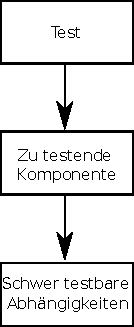
\includegraphics[width=0.2205\textwidth]{pics/humble_object_pattern_01.pdf}
     }
     \hfill
     \subfloat[\label{fig:humble_02}]{
       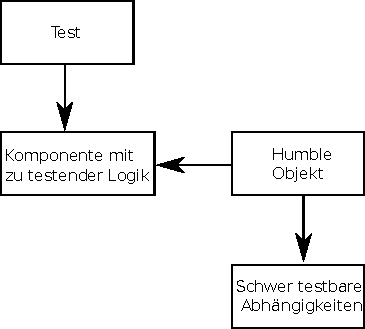
\includegraphics[width=0.598\textwidth]{pics/humble_object_pattern_02.pdf}
     }
     \hfill
     \caption[Veranschaulichung des \textit{Humble Object Pattern}.]{Veranschaulichung des Humble Object Pattern. Abbildung \sref{fig:humble_01} zeigt die Ausgangssituation, in \sref{fig:humble_02} wird das Ergebnis dargestellt. Die tatsächliche Logik einer Komponente wird in eine neue Klasse ausgelagert und dort isoliert getestet.}
     \label{fig:humble_object_pattern}
\end{minipage}
   \end{figure}


In \cite{xUnit_Test_Patterns_Refactoring} beschreibt Meszaros drei verschiedene Möglichkeiten, die Referenz eines \textit{Humble Objekts} auf die Komponente, die die ausgelagerte Logik enthält, zu realisieren. Die simpelste Möglichkeit ist, für jede Methode einer Klasse eine weitere Methode zu erstellen, die die tatsächliche Logik enthält. Hierbei ist keine Referenz zu anderen Klassen notwendig, allerdings leidet die Übersichtlichkeit und Klassen können schnell sehr groß werden. Bei Variante zwei wird für jede Klasse, die zu testende Funktionalität enthält, eine neue Klasse erstellt und die zu testenden Methoden mit der tatsächlichen Logik innerhalb dieser platziert. Das \textit{Humble Objekt} hält dann eine Referenz auf diese Klasse. Die letzte Möglichkeit erweitert dieses Vorgehen noch und sieht vor, das \textit{Humble Objekt} als abgeleitete Klasse der Klassen mit ausgelagerter Funktionalität zu realisieren. Somit können die Methoden mit ausgelagerter Funktionalität in verschiedenen Klassen verwaltet werden. Das \textit{Humble Objekt} muss lediglich von diesen Klassen erben und keine Referenzen speichern.

Hinsichtlich des konkreten Projekts ergeben sich durch eine Gegenüberstellung der beiden soeben vorgestellten Herangehensweisen Vor- und Nachteile für beide Seiten. Das Hinzufügen einer Komponente zu einem leeren Spielobjekt führt zu weniger Klassen, als es bei der Anwendung des \textit{Humble Object Pattern} der Fall wäre. Dort wird für jede zu testende Klasse eine weitere benötigt, wodurch sich die Anzahl notwendiger Klassen verdoppelt. Dies resultiert in unübersichtlicheren Strukturen. Darüber hinaus ist es oftmals nicht ohne Weiteres möglich, anwendungsbezogenen Quellcode von äußeren Abhängigkeiten klar abzugrenzen. Die Auslagerung der für die Logik verantwortlichen Codefragmente in eigene Methoden erfordert in manchen Fällen einen nicht unerheblichen Aufwand und führt auch hier zu unübersichtlicheren Strukturen mit stellenweise viel Quellcode, der lediglich die Kommunikation zwischen dem \textit{Humble Objekt} und dem ausgelagerten Code steuert. Diese Kommunikation führt neben einem höheren Entwicklungsaufwand auch zu Einbußen hinsichtlich der Performanz des Gesamtsystems. Ein positiver Aspekt des \textit{Humble Object Pattern} ist die Tatsache, dass mit Hilfe von Standardverfahren und Werkzeugen verschiedene Testüberdeckungsmetriken berechnet werden können. Doch selbst dieses Argument wird durch Unity eigene Besonderheiten abgeschwächt, die eine automatisierte Auswertung der Testüberdeckung erschweren. Nach Abwägung aller Vor- und Nachteile wurde daher entschieden, die zu testenden Komponenten direkt zu testen und daraus entstehende Nachteile bewusst in Kauf zu nehmen. 


%- Direkt die Klassen testen (wie kommt man mit MonoBehaviours klar?) => Leere Spielobjekte erstellen und Komponenten hinzufügen. 
% - Schneller!
%- Keine redundanten Klassen
%- Weniger Codevolumen
%- Übersichtlicherer Code
%- Teilweise sehr kompliziert, den Code auszulagern (Abhängigkeiten, siehe Zugriff auf transform-Objekte usw. ...)
%- 
%\linebreak
%- Funktionalen Code auslagern in extra Klassen -> \textit{Humble Object Pattern} [Vgl. \cite{xUnit_Test_Patterns_Refactoring}]
%
%- Metriken zur Code-Coverage einfacher möglich
%- 



%\subsubsection{Gewähltes Vorgehen und Begründung}
%Evtl ganz rauswerfen. Steht alles schon im vorhergehenden Kapitel. 

%
%\subsubsection{Unlösbare Probleme und mögliche Alternativen}
%
%- Serialisierung automatisiert testen. -> Es werden LevelElemente serialisiert, und diese existieren nicht wenn die Unity Engine nicht läuft (also im isolierten automatischen Test)! Diese lassen sich auch nicht im Testfall erzeugen, da es MonoBehaviours sind! Deserialisieren und dann serialisieren funktioniert auch nicht, da beim Deserialisieren nur LevelElementDATA Objekte deserialisiert/wiederhergestellt werden, und diese dann mithilfe der Unity Engine (die beim isolierten Test nicht vorhanden ist) in LevelElemente umgewandelt werden! Gleiches Problem -> die LevelElementDATA Objekte können nicht in LevelElements überführt werden, die aber zur Serialisierung notwendig sind!
%
%- LevelController, ...

%\subsubsection{Ausgewählte Problemstellungen}

\subsubsection{Übersicht bezüglich der Testabdeckung}

\begin{table}[b!]
\caption[abc]{Darstellung verschiedener Eigenschaften sowie selbst definierter Metriken für verschiedene Komponenten des Projekts.}
\begin{center}
\begin{tabular}{|l||l|l|l|l|l||l|l|}
\hline
  Funktionalität & Klassen $k$ & Methoden $m$ & $LOC_F$ & Testfälle $t$ & $LOC_T$ & $\frac{t}{m}$ & $\frac{LOC_T}{LOC_F}$ \\
  \hline
  Audio & 11 & 21 & 437 & 0 & 0 & 0,00 & 0,00 \\
  Kamera & 1 & 1 & 47 & 0 & 0 & 0,00 & 0,00 \\
  Anzeige & 3 & 0 & 131 & 0 & 0 & 0,00 & 0,00 \\
  Hauptmenü & 4 & 11 & 162 & 0 & 0 & 0,00 & 0,00\\
  Spielersteuerung & 2 & 11 & 284 & 0 & 0 & 0,00 & 0,00\\
  Level Elemente & 9 & 15 & 419 & 20 & 289 & 1,33 & 0,69 \\
  Levelaufbau & 10 & 40 & 910 & 60 & 1.047 & 1,68 & 1,50\\
  Level-Editor & 10 & 37 & 1.282 & 0 & 0 & 0,00 & 0,00\\
  Level speichern/ &&&&&&&\\
  Level laden & 3 & 6 & 448 & 4 & 760 & 0,67 & 1,70\\
  Waffen & 10 & 16 & 468 & 0 & 0 & 0,00 & 0,00\\
  Gegner und &&&&&&&\\
  KI Verhalten & 11 & 34 & 1.089 & 0 & 0 & 0,00 & 0,00\\
  KI Schnittstelle & 4 & 13 & 551 & 0 & 0 & 0,00 & 0,00\\
  Pfadfindung & 10 & 12 & 623 & 12 & 346 & 1,00 & \\
  Fibonacci-Heap & 2 & 12 & 215 & 20 & 379 & 1,67 & 1,76\\  
  Hilfsklassen & 4 & 14 & 238 & 40 & 237 & 2,86 & 1,00\\  
  \hline
\end{tabular}
\label{tab:testabdeckung}
\end{center}
\end{table}

Wie bereits in Kapitel \ref{chapter:mono_beh_testen_loesungen} beschrieben, erschwert das gewählte Vorgehen zur Entwicklung der Modultests die automatisierte Auswertung hinsichtlich verschiedener Metriken. Es wurden daher eigene Maße definiert, um eine Aussage bezüglich der Testabdeckung innerhalb der verschiedenen Komponenten des Projekts zu erhalten und diese untereinander vergleichen zu können. Die manuelle Auswertung dieser Maße ist in Tabelle \ref{tab:testabdeckung} dargestellt. In Spalte eins sind die verschiedenen Komponenten aufgeführt. Hierzu werden Klassen mit identischen Einsatzbereichen zu Oberkategorien zusammengefasst. Die Spalten zwei, drei und vier geben Auskunft über die Anzahl Klassen, Anzahl Methoden und Anzahl geschriebener Zeilen Quellcode innerhalb dieser Komponenten. In Spalte drei werden lediglich öffentlich zugreifbare Methoden berücksichtigt, da Implementierungsdetails innerhalb privater Methoden für den Benutzer einer Klasse nicht relevant sind. Da die nachfolgende Spalte einen Überblick hinsichtlich des Codevolumens innerhalb einer Komponente gibt, werden hierbei wiederum alle Funktionalitäten jeglicher Zugriffsmodifikatoren berücksichtigt. In den folgenden beiden Spalten werden die Anzahl Testfälle sowie die Anzahl geschriebener Zeilen Quellcode innerhalb dieser Testfälle aufgelistet. Parametrisierte Tests, also Testmethoden gleicher Struktur, die mit unterschiedlichen Argumenten aufgerufen werden, werden sowohl bei der Bestimmung der Anzahl Testfälle als auch in Bezug auf den Umfang des Quellcodes als separate Tests betrachtet. Die letzten zwei Spalten zeigen selbst definierte Metriken, die zum einen das Verhältnis existierender Testfälle zu vorhandenen öffentlichen Methoden und zum andern den Quotienten aus der Anzahl Zeilen zur Erstellung der Testfälle und Anzahl Zeilen der tatsächlichen Funktionalitäten wiedergeben. 

Hierbei ist zu erkennen, dass für nur fünf von möglichen fünfzehn Komponenten überhaupt Testfälle existieren. Dies lässt sich durch die Bedeutung dieser Komponenten im Projekt erklären. Die Kategorien Level Elemente, Levelaufbau, Level speichern und Level laden, Pfadfindung und Fibonacci-Heap stellen Grundfunktionalitäten der Software dar, auf denen viele andere wichtige Entwicklungen aufbauen. Die im Verhältnis meisten Testfälle pro öffentlicher Methode sind in den Hilfsklassen zu finden. Der Grund hierfür ist die Verwendung vieler parametrisierter Tests, deren primäres Ziel die Überprüfung der zu testenden Methoden mit unterschiedlichen Argumenten darstellt. Das Verhältnis von geschriebenen Zeilen Testcode zur Anzahl funktionaler Zeilen ist bei der Fibonacci-Heap Datenstruktur am höchsten. Aufgrund des relativ geringen Umfangs der tatsächlichen Funktionalität genügen hierzu vergleichsweise unterdurchschnittlich viele Zeilen Testcode. 





% Die Aussagekraft der in Tabelle \ref{tab:testabdeckung} dargestellten Zahlen muss allerdings auch

%- Unity hat test coverage tool eingestellt usw. 




%- Testabdeckung (Automatisiert nicht möglich, Gründe, Vom Markt genommen, ...)
%- Offizielles Statement von Unity zu Testabdeckung/Testen
%- Was konnte denn getestet werden, was nicht? Welche Klassen sind ganz gut abgedeckt, welche überhaupt nicht? Gründe dafür nennen!

\subsection{Manuelle Tests}

Neben automatisierten Modultests ist auch die Durchführung manueller Tests ein wichtiger Bestandteil des Projekts. Dies ist zum einen in Szenarien notwendig, in denen automatisierte Tests aufgrund vieler komplexer Abhängigkeiten nur schwer erstellbar sind. Zum anderen eignen sich manuelle Tests zur Überprüfung von Spielabläufen, in denen das Zusammenspiel mehrerer Komponenten miteinander untersucht werden muss. Da die manuelle Begutachtung sehr schnell und unkompliziert ausgeführt werden kann, stellt dieses Vorgehen eine echte Alternative zum Schreiben von \textit{PlayMode} Tests dar. Im Folgenden sind die wichtigsten Funktionalitäten stichpunktartig aufgeführt, deren korrektes Verhalten durch manuelle Tests überprüft wurde: 

\begin{itemize}
\item Steuerung des Spielers: Der Spieler bewegt sich entsprechend der getätigten Eingaben und kann nicht durch Wände hindurchgehen. Das Ablegen und Aufheben von Waffen sowie das Sammeln von Munition funktioniert wie erwartet. Ein Spieler kann nicht durch geschlossene Türen oder Wände hindurchschießen.  
\item Level speichern und laden: Ein aktueller Spielstand kann per Knopfdruck auf zweierlei Arten gesichert und zu einem späteren Zeitpunkt über das Hauptmenü korrekt wiederhergestellt werden. 
\item Gegnerverhalten, Pfadfindung und Audio: Gegner reagieren auf Geräusche in ihrer Umgebung sowie auf Sichtkontakt mit dem Spieler. Des Weiteren verfolgen Gegner den Spieler, allerdings sind diese nicht allwissend und brechen die Verfolgung bei gewissen Bedingungen wieder ab. Anschließend kehren sie zu ihrer ursprünglichen Route zurück. 
\item Level-Editor: Verschiedene Level Elemente (Wände, Türen) sowie Waffen können frei platziert werden. Die Größe eines Levels kann beliebig festgelegt werden. Ein erstelltes Level kann gespeichert und zu einem späteren Zeitpunkt über das Hauptmenü wieder geladen werden. Es können Gegner verschiedenen Schwierigkeitsgrades frei positioniert und mit Waffen ausgestattet werden. Alle platzierten Komponenten können während der Erstellung auch wieder entfernt werden. 
\end{itemize}

Da manuelle Tests immer von Menschen durchgeführt werden, sind diese deutlich fehleranfälliger als automatisiert prüfende Testverfahren. Hinsichtlich des konkreten Projekts stellen diese trotz allem eine einfache Möglichkeit dar, die Funktionalität und das Zusammenspiel verschiedener Komponenten auch bei häufigen Änderungen im Zuge des Entwicklungsprozesses mit geringem Aufwand überprüfen zu können. 

%- Level serialisieren/deserialisieren und manuelle vergleichen.
%- Waffen aufheben, schießen (durch geschlossene Türen, Wände, ...) 
%- => Da wo automatisierte Tests nicht möglich waren, musste manuell geprüft werden!